\question{}

\begin{enumerate}
    \item \textbf{توضیح الگوریتم و عملکرد مدار:}
          این مدار در واقع یک محاسبه‌گر توان ۲ است که عدد $2^{\text{\lr{in}}_\text{\lr{0}}}$ را محاسبه می‌کند. الگوریتم مدار به این صورت است که ابتدا منتظر می‌ماند تا سیگنال \lr{Start} فعال شود. با فعال شدن این سیگنال، مقدار ورودی ۳ بیتیِ $\text{\lr{in}}_\text{\lr{0}}$ را در شمارنده‌ی \lr{R0} ذخیره کرده و همزمان مقدار ثابت 1 (یا همان \lr{0b00000001}) را در ثبات شیفت‌دهنده‌ی \lr{R1} قرار می‌دهد. سیگنال اعلام پایان کار (\lr{RE}) نیز در همین مرحله صفر می‌شود.

          در مرحله‌ی بعد، سیستم وارد یک حلقه‌ی تکرار می‌شود و تا زمانی که مقدار \lr{R0 > 0} باشد، در هر چرخه ثبات \lr{R1} را یک واحد به سمت چپ شیفت می‌دهد (ضرب در ۲) و همزمان یک واحد از شمارنده‌ی \lr{R0} کم می‌کند. وقتی شمارنده به صفر رسید، حلقه پایان می‌یابد. در این لحظه، ثبات \lr{R1} دقیقاً به تعداد $\text{\lr{in}}_\text{\lr{0}}$ بار به چپ شیفت پیدا کرده است. در نهایت، سیستم مقدار محاسبه شده در \lr{R1} را در رجیستر خروجی \lr{Y} بارگذاری کرده و با یک کردن سیگنال \lr{RE} (یا همون \lr{Done})، پایان عملیات و معتبر بودن خروجی را اعلام می‌کند و به حالت اولیه بازمی‌گردد.

    \item \textbf{بررسی چرخه‌دقیقه‌ای و دیاگرام زمانی:}
          برای بررسی رفتار چرخه‌دقیق مدار، جدول شبیه‌سازی زیر آماده شده است. مقادیر وضعیت سیستم و ثبات‌ها در هر چرخه‌ی ساعت (\lr{Clk}) قابل استخراج و ثبت می‌باشد:

          \begin{table}[H]
              \centering
              \caption{جدول شبیه‌سازی چرخه‌دقیق (\lr{Cycle-Accurate}) سامانه}
              \vspace{0.5em}
              \begin{tabular}{|c|c|c|c|c|c|c|}
                  \hline
                  \textbf{\lr{ASM Block}} & \textbf{\lr{Y}} & \textbf{\lr{RE}} & \textbf{\lr{R1}} & \textbf{\lr{R0}} & \textbf{\lr{Start}} & \textbf{\lr{Clk}} \\
                  \hline
                  Init                    & --              & --               & --               & --               & 1                   & 1                 \\ \hline
                  Init                    & --              & 0                & 1                & 5                & 0                   & 2                 \\ \hline
                  Calculate               & --              & 0                & 2                & 4                & 0                   & 3                 \\ \hline
                  Calculate               & --              & 0                & 4                & 3                & 0                   & 4                 \\ \hline
                  Calculate               & --              & 0                & 8                & 2                & 0                   & 5                 \\ \hline
                  Calculate               & --              & 0                & 16               & 1                & 0                   & 6                 \\ \hline
                  Calculate               & --              & 0                & 32               & 0                & 0                   & 7                 \\ \hline
                  Done                    & 32              & 1                & 32               & 0                & 0                   & 8                 \\ \hline
                  Init                    & 32              & 1                & 32               & 0                & 0                   & 9                 \\ \hline
              \end{tabular}
          \end{table}

          \pagebreak

          \begin{figure}[H]
              \centering
              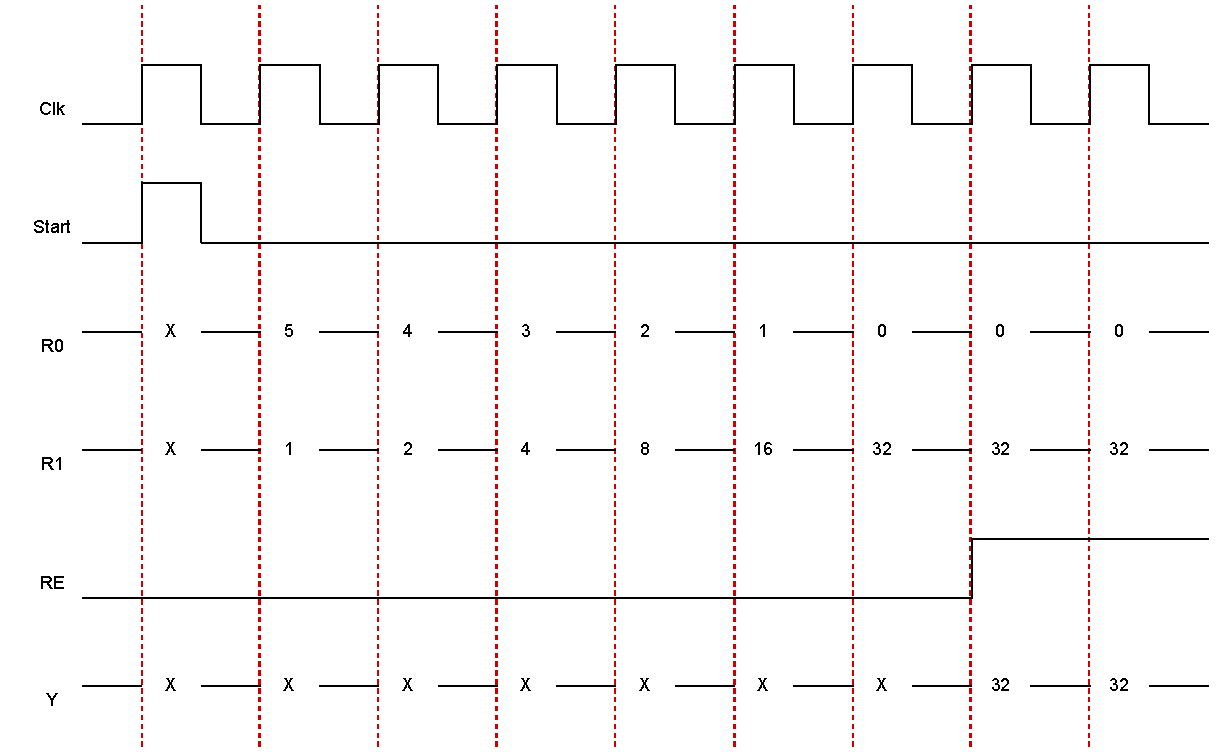
\includegraphics[width=1.0\textwidth]{assets/Q2-Diagram.pdf}
              \caption{دیاگرام زمانی فرآیند محاسبه}
          \end{figure}

    \item \textbf{سنتز مدار به واحد کنترل و مسیر داده:}
          \textbf{سنتز مسیر داده (\lr{Data Path}):}
          \begin{figure}[H]
              \centering
              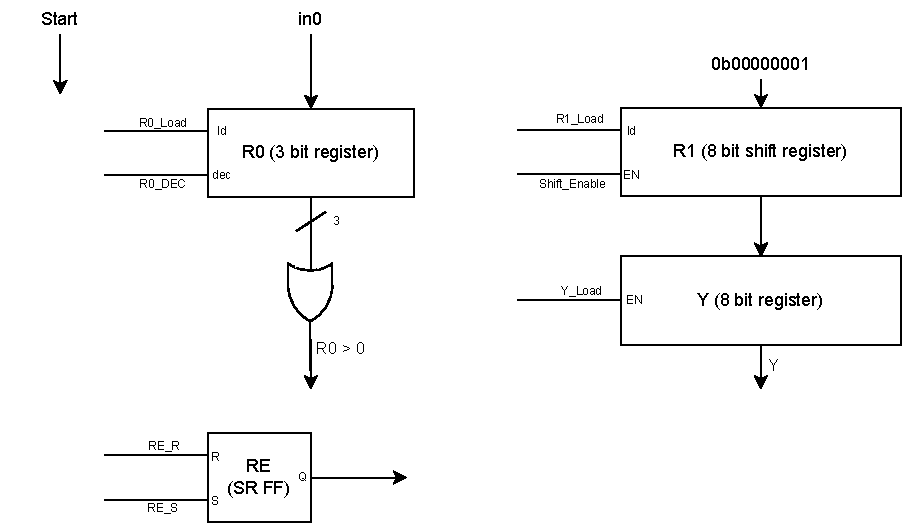
\includegraphics[width=0.7\textwidth]{assets/Q2-synthes-DP.pdf}
              \caption{بخش مسیر داده (\lr{Data Path})}
          \end{figure}
          در مسیر داده به اجزای زیر نیاز داریم:
          \begin{itemize}
              \item شمارنده \lr{R0}: یک ثبات ۳ بیتی با قابلیت بارگذاری موازی (پایه‌ی \lr{Load} برای دریافت $\text{\lr{in}}_\text{\lr{0}}$) و شمارش رو به پایین (پایه‌ی \lr{DEC}). همچنین یک گیت \lr{OR} برای تشخیص شرط $\text{\lr{R0}} > 0$ از روی بیت‌های آن لازم است.
              \item ثبات \lr{R1}: یک \lr{Shift Register} هشت بیتی با قابلیت بارگذاری موازی (پایه‌ی \lr{Load} برای دریافت مقدار ثابت \lr{0b00000001}) و شیفت به چپ (پایه‌ی \lr{Shift\_Enable}).
              \item رجیستر \lr{Y}: یک ثبات ۸ بیتی با پایه‌ی فعال‌ساز (\lr{Y\_Load}) برای نگهداری نتیجه نهایی.
              \item سیگنال \lr{RE}: یک فلیپ‌فلاپ نوع \lr{SR} برای تنظیم وضعیت پرچمِ پایان عملیات.
          \end{itemize}

          \textbf{سنتز واحد کنترل (\lr{Control Unit}):}
          بر اساس نمودار \lr{ASM} داده شده، سیستم را می‌توان به ۳ بلاک \lr{Init}، \lr{Calculate} و \lr{Done} تقسیم کرد.

          \begin{figure}[H]
              \centering
              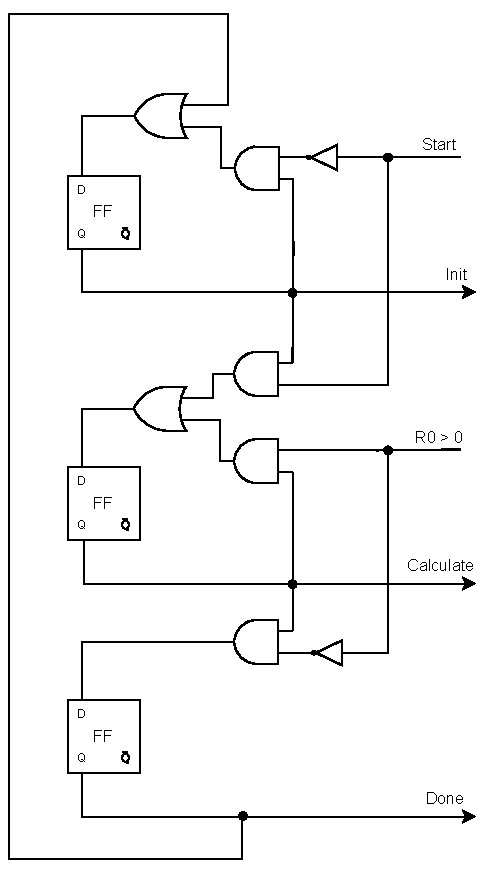
\includegraphics[width=0.5\textwidth]{assets/Q2-synthes-CU.pdf}
              \caption{واحد کنترل (\lr{Control Unit})}
          \end{figure}
          با استفاده از روش \lr{One-Hot}، برای سه حالت موجود به ۳ فلیپ‌فلاپ \lr{D} نیاز داریم که معادلات انتقال حالت آن‌ها به شرح زیر است:
          \begin{align*}
              \text{\lr{Init}}^{+}      & = (\text{\lr{Init}} \cdot \overline{\text{\lr{Start}}}) + \text{\lr{Done}}                        \\
              \text{\lr{Calculate}}^{+} & = (\text{\lr{Calculate}} \cdot (\text{\lr{R0}} > 0)) + (\text{\lr{Init}} \cdot \text{\lr{Start}}) \\
              \text{\lr{Done}}^{+}      & = \text{\lr{Calculate}} \cdot \overline{(\text{\lr{R0}} > 0)}
          \end{align*}

          همچنین سیگنال‌های فرمان مسیر داده (\lr{Command Signals}) که توسط واحد کنترل تولید می‌شوند، بر اساس شرط‌های موجود در بلوک‌های \lr{ASM} به این شکل استخراج می‌شوند:
          \begin{align*}
              \text{\lr{R0\_Load}} = \text{\lr{RE\_R}} = \text{\lr{R1\_Load}} & = \text{\lr{Init}} \cdot \text{\lr{Start}}         \\
              \text{\lr{Shift\_Enable}} = \text{\lr{R0\_DEC}}                 & = \text{\lr{Calculate}} \cdot (\text{\lr{R0}} > 0) \\
              \text{\lr{Y\_Load}} = \text{\lr{RE\_S}}                         & = \text{\lr{Done}}
          \end{align*}
\end{enumerate}